\documentclass[11pt,class=report,crop=false]{standalone}
\usepackage[screen]{../python}


\begin{document}


%====================================================================
\chapitre{Dérivée -- Zéros de fonctions}
%====================================================================

\index{derivee@dérivée}

\index{zeros@zéros}

\objectifs{Nous étudions les fonctions : 
le calcul de la dérivée d'une fonction, 
le tracé du graphe et de tangentes,
et enfin la recherche des valeurs en lesquelles la fonction s'annule.}


%%%%%%%%%%%%%%%%%%%%%%%%%%%%%%%%%%%%%%%%%%%%%%%%%%%%%%%%%%%%%%%%
%%%%%%%%%%%%%%%%%%%%%%%%%%%%%%%%%%%%%%%%%%%%%%%%%%%%%%%%%%%%%%%%

\begin{cours}[Dérivée]
Par définition le nombre dérivé de $f$ en $a$ (s'il existe) est:
$$f'(a) = \lim_{h\to0} \frac{f(a+h)-f(a)}{h}.$$

Dans cette fiche nous supposerons que toutes les dérivées étudiées existent.

Voici l'interprétation géométrique du nombre dérivé : $f'(a)$ est le coefficient directeur de la tangente\index{tangente}
au graphe de $f$ au point d'abscisse $a$.

\myfigure{1.2}{
\tikzinput{fig-derivee-1}
}

\end{cours}


\begin{cours}[Fonction lambda]
	
\index{fonction lambda}
\index{lambda@\ci{lambda}}
	
Une fonction lambda (lettre grecque $\lambda$) est une façon simple de définir une fonction en \Python{} qui s'apparente à une fonction mathématique. Par
exemple :
\mycenterline{\ci{f = lambda x: x**2}}
Cela définit une fonction \Python{} \ci{f} qui correspond à la fonction mathématique $f$ définie par $f : x \mapsto x^2$.
Ainsi \ci{f(2)} renvoie \ci{4}, \ci{f(3)} renvoie \ci{9}\ldots

C'est une alternative condensée au code suivant :
\begin{center}
\begin{minipage}{0.6\textwidth}
\begin{lstlisting}
def f(x):
    return x**2
\end{lstlisting} 
\end{minipage}
\end{center}

\bigskip

Une fonction est un objet \Python{} comme un autre. Elle peut donc être utilisée dans le programme comme dans l'exemple suivant qui teste si $f(a)>f(b)$ :

\begin{center}
\begin{minipage}{0.6\textwidth}
\begin{lstlisting}
def est_plus_grand(f,a,b):
    if f(a) > f(b):
        return True
    else:
        return False  
\end{lstlisting} 
\end{minipage}
\end{center}


Pour les deux fonctions \ci{f} définies au-dessus (soit à l'aide de \ci{lambda}, soit à l'aide de \ci{def}) alors
\mycenterline{\ci{est_plus_grand(f,1,2)}}
renvoie \og{}Faux\fg{}.

\`A l'aide des fonctions lambda on peut aussi se permettre de ne pas donner de nom à une fonction, comme ci-dessous avec la fonction $x \mapsto \frac1x$. Alors
\mycenterline{\ci{est_plus_grand(lambda x:1/x,1,2)}}
qui renvoie \og{}Vrai\fg{} (\ci{lambda x:1/x} joue le rôle de \ci{f}).
\end{cours}



%%%%%%%%%%%%%%%%%%%%%%%%%%%%%%%%%%%%%%%%%%%%%%%%%%%%%%%%%%%%%%%%
% Activité 1
%%%%%%%%%%%%%%%%%%%%%%%%%%%%%%%%%%%%%%%%%%%%%%%%%%%%%%%%%%%%%%%%

\begin{activite}[Calcul de la dérivée en un point]

\objectifs{Objectifs : calculer une valeur approchée de la dérivée en un point.}

On va calculer une valeur approchée du nombre dérivé $f'(a)$ en calculant le taux d'accroissement $\frac{f(a+h)-f(a)}{h}$ avec $h$ suffisamment petit.

\begin{enumerate}
  \item Définis la fonction $f$, $x \mapsto x\sqrt{1-x}$.
  Deux méthodes : soit à l'aide de \ci{def f(x):...}, soit par 
  \ci{f = lambda x:...} \ 
  Calcule les valeurs approchées de $f(k)$ pour $k \in \{0,1,2,\ldots,5\}$.
  
  \item Programme une fonction \ci{derivee(f,a)} qui calcule une valeur approchée de la dérivée de $f$ en $a$ par la formule
  $$f'(a) \simeq \frac{f(a+h)-f(a)}{h}$$
  en prenant par exemple pour valeur $h=0.0001$.
  
  
  Pour la fonction $f : x\mapsto x^3$, compare 
  la valeur approchée en $a$ que tu obtiens avec la valeur exacte de $f'(k)$ pour $k \in \{0,1,2,\ldots,5\}$.  
  Diminue la valeur de $h$ pour obtenir une meilleure approximation.
  
\end{enumerate} 

\end{activite}


%%%%%%%%%%%%%%%%%%%%%%%%%%%%%%%%%%%%%%%%%%%%%%%%%%%%%%%%%%%%%%%%
% Activité 2
%%%%%%%%%%%%%%%%%%%%%%%%%%%%%%%%%%%%%%%%%%%%%%%%%%%%%%%%%%%%%%%%

\begin{activite}[Graphe d'une fonction et tangente]

\objectifs{Objectifs : tracer le graphe d'une fonction ainsi que des tangentes.}


Soit $f : [a,b] \to \Rr$ une fonction. Son graphe $G_f$ est :
$$G_f = \left\{ \big(x,f(x)\big) \mid x \in [a,b] \right\}$$

\myfigure{1.2}{
\tikzinput{fig-derivee-2}
}

\begin{enumerate}

  \item \textbf{Calculer des points.}
  Soit $f$ une fonction définie sur un intervalle $[a,b]$. 
  On divise l'intervalle $[a,b]$ en $n$ sous-intervalles de longueur $\frac{b-a}{n}$ en définissant :
  $$x_k = a + k \frac{b-a}{n}.$$
  
\myfigure{0.7}{
\tikzinput{fig-derivee-3}
}  

  Programme une fonction \ci{graphe(f,a,b,n)} qui calcule et renvoie la liste des points $\big(x_k,f(x_k)\big)$ pour $k = 0,\ldots,n$.
  
 \myfigure{0.9}{
\tikzinput{fig-derivee-4}
}   

   Par exemple pour \ci{f = lambda x: x*x} alors
   \ci{graphe(f,0,2,4)} renvoie la liste :
   \mycenterline{\ci{[(0, 0), (0.5, 0.25), (1.0, 1.0), (1.5, 2.25), (2.0, 4.0)]}}
  
  \item \textbf{Afficher des points.}    
  Programme une fonction \ci{afficher_points(points)} qui affiche une liste de points. 
  
  \emph{Indications.} Tu peux utiliser le module \ci{tkinter}  (ou bien le module \ci{matplotlib}). Tu peux utiliser une variable \ci{echelle} pour contrôler la taille de l'affichage.
  Les figures ci-dessous sont tracées pour la fonction $f$ définie par $f(x)= \sqrt{x}$ sur l'intervalle $[0,4]$.
   
\begin{center}
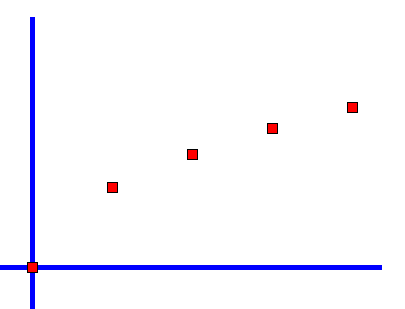
\includegraphics[scale=0.3]{ecran-graphe-1}
\end{center}
  
  \item \textbf{Tracer le graphe.}
  Améliore la fonction précédente pour écrire  une fonction \ci{tracer_graphe(f,a,b)} qui trace le graphe de $f$.
  
  \emph{Indications.} Il suffit de relier $n$ points du graphe entre eux pour $n$ assez grand (avec $5$ points à gauche et $20$ points à droite).
  
\begin{center}
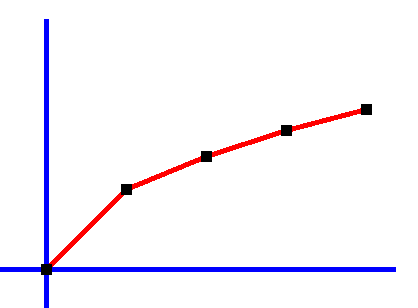
\includegraphics[scale=0.3]{ecran-graphe-2} \qquad
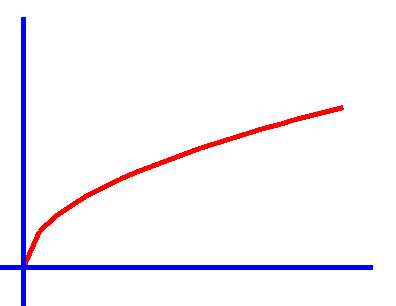
\includegraphics[scale=0.3]{ecran-graphe-3}
\end{center}

  
  \item \textbf{Tracer une tangente.}
  
  Trace la tangente au graphe au point $(a,f(a))$ par une fonction \ci{tracer_tangente(f,a)}.
  
\begin{center}
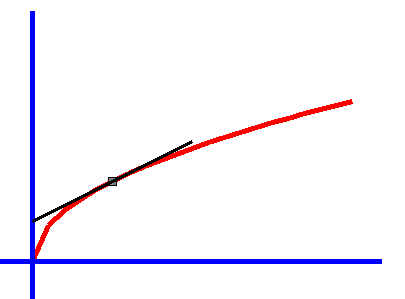
\includegraphics[scale=0.3]{ecran-graphe-4}
\end{center}  
  
  \emph{Indications.}
  On se place au point $(x,y) = (a,f(a))$. En ce point la pente de la tangente est donnée par $f'(a)$. En posant 
  $$dx = 1 \quad \text{ et } \quad dy = f'(a)$$
  alors on représente une demi-tangente par le segment reliant
  $(x,y)$ à $(x+dx,y+dy)$. L'autre demi-tangente est représentée par le segment reliant 
  $(x,y)$ à $(x-dx,y-dy)$.

  \myfigure{1.3}{
\tikzinput{fig-derivee-5}
}  
  
  
  

  
 
  
  
\end{enumerate} 


Cette activité peut être l'occasion d'utiliser les arguments optionnels,
par exemple au lieu de définir la fonction \ci{tracer_graphe()} par l'entête:
\mycenterline{\ci{def tracer_graphe(f,a,b):}}
et d'avoir des variables locales \ci{n} et \ci{echelle}, tu peux définir ta fonction par :
\mycenterline{\ci{def tracer_graphe(f,a,b,n=20,echelle=50):}}
Ce qui permet d'avoir une valeur de \ci{n} et de \ci{echelle} par défaut, en conservant la possibilité de les changer. Des appels possibles sont :
\begin{itemize}
  \item \ci{tracer_graphe(f,a,b)} ;
  \item \ci{tracer_graphe(f,a,b,n=100)}  pour tracer plus de points ;
  \item \ci{tracer_graphe(f,a,b,echelle=10)} pour changer l'échelle.
\end{itemize}
\end{activite}



%%%%%%%%%%%%%%%%%%%%%%%%%%%%%%%%%%%%%%%%%%%%%%%%%%%%%%%%%%%%%%%%
% Activité 3
%%%%%%%%%%%%%%%%%%%%%%%%%%%%%%%%%%%%%%%%%%%%%%%%%%%%%%%%%%%%%%%%

\begin{cours}[Dichotomie]

\index{dichotomie}

Le méthode de dichotomie est basée sur cette version du théorème des valeurs intermédiaires.

\medskip

\textbf{Théorème.} Soit $f : [a,b] \to \Rr$ une fonction continue.
Si $f(a)$ et $f(b)$ sont de signes contraires, alors $f$ s'annule au moins une fois sur l'intervalle $[a,b]$. Autrement dit, il existe $\ell\in[a,b]$ tel que $f(\ell)=0$.

\medskip

\myfigure{1}{
\tikzinput{fig_zeros01}\quad
\tikzinput{fig_zeros02}
}
\medskip 

\textbf{Principe de la dichotomie} ($\delta\iota\chi o \tau o\mu\iota\alpha$
signifie \og{}coupé en deux\fg{}).
On sait que notre fonction $f$ s'annule sur $[a,b]$. On calcule $f\left(\frac{a+b}{2}\right)$, c'est-à-dire l'image du milieu du segment $[a,b]$. On cherche ensuite où $f$ peut s'annuler par rapport à ce milieu :
\begin{itemize}
  \item Si $f(a)$ et $f\left(\frac{a+b}{2}\right)$ sont de signes contraires alors $f$ s'annule sur
  $\left[ a, \frac{a+b}{2}\right]$,
  
  \item sinon $f$ s'annule sur
  $\left[\frac{a+b}{2},b\right]$.
\end{itemize}

\myfigure{1}{
\tikzinput{fig_zeros03}\quad
\tikzinput{fig_zeros04}
}


On recommence l'opération sur l'intervalle $\left[ a, \frac{a+b}{2}\right]$ ou bien sur l'intervalle $\left[\frac{a+b}{2},b\right]$.

Remarques :
\begin{itemize}
  \item $f(a)$ et $f(b)$ sont de signes contraires  si et seulement si $f(a) \times f(b) \le 0$.
  \item On va construire des intervalles de plus en plus petits qui contiennent une solution $\ell$, de $f(\ell) = 0$. On obtient donc un encadrement de $\ell$ (mais pas sa valeur exacte).
  \item Il se peut que $f$ s'annule plusieurs fois, mais la méthode de dichotomie ne fournit l'encadrement que d'une seule solution.
  \item Pour expliquer la partie \og{}si\fg{} du principe de la dichotomie, on applique le théorème des valeurs intermédiaires sur 
$\left[ a, \frac{a+b}{2}\right]$. Pour expliquer la partie \og{}sinon\fg{}, on remarque d'abord que 
$f(b)$ et $f\left(\frac{a+b}{2}\right)$ doivent être de signes contraires, puis on applique le théorème des valeurs intermédiaires.
\end{itemize}

\begin{exemple}
On cherche \og{}à la main\fg{} une valeur approchée de $\sqrt{2}$.

\begin{itemize}
  \item Soit $f$ définie par $f(x)=x^2-2$. On se place sur l'intervalle $[1,2]$.
  \item Comme $f(1)=-1\le0$ et $f(2)=2\ge0$ et que $f$ est continue alors $f$ s'annule sur l'intervalle $[1,2]$ par le théorème des valeurs intermédiaires. Bien sûr, ici $f$ s'annule en $\ell = \sqrt{2}$. Pour l'instant on a prouvé : $1 \le \sqrt 2 \le 2$.
  \item On divise l'intervalle $[1,2]$ en deux parties, le milieu étant $\frac32$, on calcule :
  $$f\left(\frac32\right)= \left(\frac32\right)^2-2 = \frac14 \ge 0.$$
  Donc sur le demi-intervalle $[1,\frac32]$ on a $f(1) \le 0$ et $f(\frac32) \ge 0$, et c'est bien là que $f$ s'annule. Autrement dit 
  $1 \le \sqrt{2} \le \frac32$. C'est un encadrement deux fois plus précis qu'auparavant.
  
  \item On divise l'intervalle $[1,\frac32]$ en deux parties, le milieu étant $\frac54$, on calcule :
  $$f\left(\frac54\right)= \left(\frac54\right)^2-2 = -\frac{7}{16} \le 0.$$
  Donc sur le demi-intervalle $[\frac54,\frac32]$ on a 
  $f(\frac54) \le 0$ et $f(\frac32) \ge 0$, ainsi 
  $\frac54 = 1.25 \le \sqrt{2} \le \frac32 = 1.5$.
  
  \item On continue ainsi, on obtient des intervalles $[a_i,b_i]$ de plus en plus petits qui encadrent $\sqrt2$ :

$$
\begin{array}{ll}
  a_0 = 1      & b_0 = 2 \\
  a_1 = 1      & b_1 = 1.5 \\
  a_2 = 1.25   & b_2 = 1.5 \\
  a_3 = 1.375  & b_3 = 1.5 \\
  a_4 = 1.375  & b_4 = 1.4375 \\
  a_5 = 1.40625 & b_5 = 1.4375 \\
  a_6 = 1.40625 & b_6 = 1.421875 \\
  a_7 = 1.4140625 & b_7 = 1.421875 \\
  a_8 = 1.4140625 & b_8 = 1.41796875 \\
\end{array}
$$

Donc en $8$ étapes on prouve que $1.4140625 \le \sqrt2 \le 1.41796875$. En particulier on obtient les deux premières décimales de $\sqrt2$ : $\sqrt2 = 1.41\ldots$
\end{itemize}

\myfigure{1}{
\tikzinput{fig_zeros05}
}

\end{exemple}

\end{cours}





\begin{activite}[Dichotomie]

\objectifs{Objectifs : trouver une solution approchée d'une équation $f(x)=0$.}

Le principe de la dichotomie se décline en l'algorithme suivant :
\begin{algorithme}
  \sauteligne 
 \begin{itemize}
   \item 
   \begin{itemize} 
       \item Entrée : une fonction $f$, un intervalle $[a,b]$ avec $f(a)\cdot f(b) \le 0$, une marge d'erreur $\epsilon$.
       \item Sortie : un intervalle $[a',b']$ tel que $|b'-a'| \le \epsilon$ sur lequel $f$ s'annule, autrement dit, il existe $a' \le \ell \le b'$ tel que $f(\ell)=0$.
     \end{itemize}
    
 
  \item Tant que $|b-a| > \epsilon$ :
   \begin{itemize}
     \item poser $c = \frac{a+b}{2}$,
     \item si $f(a) \times f(c) \le 0$, faire $b \leftarrow c$, % (on se place sur le demi-intervalle de gauche)
     \item sinon, faire $a \leftarrow c$. % (on se place sur le demi-intervalle de droite).     
     \end{itemize}   
     
     
   \item \`A la fin renvoyer $a$ et $b$ (qui encadrent la solution).
 \end{itemize}  
 \end{algorithme}



\begin{enumerate}
  \item Programme cet algorithme en une fonction \ci{dichotomie(f,a,b,epsilon)}.
  
  \item \emph{Exemples.} 
  \begin{enumerate}
   \item Trouve une valeur approchée de $\sqrt{3}$ à $10^{-3}$ près, en utilisant la fonction définie par $f(x) = x^2-3$ sur l'intervalle $[1,2]$.
    \item Trouve une valeur approchée de $\sqrt[3]{5}$, en utilisant la fonction définie par $f(x) = x^3-5$.
    \item Trouve une valeur approchée de chacune des trois solutions de l'équation $x^5-3x+1=0$.  
  \end{enumerate}
  
  \item Soit la fonction définie par $f(x) = x^2-3$ sur l'intervalle $[1,2]$. Combien faut-il d'étapes pour obtenir une approximation de $\sqrt{3}$ avec $10$ décimales exactes après la virgule ?
  
\end{enumerate} 

\end{activite}


%%%%%%%%%%%%%%%%%%%%%%%%%%%%%%%%%%%%%%%%%%%%%%%%%%%%%%%%%%%%%%%%
% Activité 4
%%%%%%%%%%%%%%%%%%%%%%%%%%%%%%%%%%%%%%%%%%%%%%%%%%%%%%%%%%%%%%%%

\begin{cours}[Méthode de Newton]

\index{methode de Newton@méthode de Newton}	
	
On va voir une autre méthode très efficace pour obtenir une valeur approchée d'une solution $\ell$
de $f(\ell)=0$.
L'idée de la méthode de Newton est d'utiliser la tangente :
\begin{itemize} 
  \item on part d'une valeur $x_0$ quelconque,
  \item on trace la tangente au graphe de $f$ au point d'abscisse $x_0$,
  \item cette tangente recoupe l'axe des abscisses en un point d'abscisse $x_1$ (figure de gauche),
  \item cette valeur $x_1$ est plus proche de $\ell$ que $x_0$,
  \item on recommence à partir de $x_1$ : on trace la tangente, elle recoupe l'axe des abscisses, on obtient une valeur $x_2$\ldots{} (figure de droite).
\end{itemize}
  
 \myfigure{1}{
\tikzinput{fig_zeros08}\quad
\tikzinput{fig_zeros10}
} 
  
On va ainsi définir une suite $(x_n)$ par récurrence.  
L'équation de la tangente en une valeur $x_n$ est donnée par 
$y-f(x_n) = f'(x_n)(x-x_n)$. En partant d'une valeur $x_0$, on obtient une formule de récurrence, pour $n\ge0$  :
$$x_{n+1} = x_n - \frac{f(x_n)}{f'(x_n)}.$$


Pour que cette méthode fonctionne il faut tout de même partir d'une valeur $x_0$ pas trop éloignée de la solution $\ell$ cherchée.

\begin{exemple}
On cherche encore \og{}à la main\fg{} une valeur approchée de $\sqrt{2}$.

\begin{itemize}
  \item Soit $f$ définie par $f(x)=x^2-2$. On a donc $f'(x) = 2x$.
  
  \item On part de $x_0=2$.
  
  \item On calcule $f(x_0) = 2$ et $f'(x_0) = 4$. Par la formule de récurrence :
  $$x_1 = x_0 - \frac{f(x_0)}{f'(x_0)} = \frac32 = 1.5$$
  
  \item On calcule $f(\frac32) = \frac14$, $f'(\frac32)=3$ et donc
  $$x_2 = x_1 - \frac{f(x_1)}{f'(x_1)} = \frac{17}{12} = 1.41666\ldots$$ 
  
  \item Puis $x_3 = 1.4142156\ldots$ qui a déjà $5$ chiffres après la virgule de corrects !
\end{itemize}

\end{exemple}

\end{cours}

\begin{activite}[Méthode de Newton]

\objectifs{Objectifs : programmer la méthode de Newton.}

\begin{algorithme}
  \sauteligne 
 \begin{itemize}
   \item 
   \begin{itemize} 
       \item Entrée : une fonction $f$, une valeur de départ $a$, un nombre d'itérations $n$.
       \item Sortie : une valeur approchée de $\ell$ tel que $f(\ell)=0$.
     \end{itemize}
    
  \item Poser $x = a$.
  \item Répéter $n$ fois:
 $$x \leftarrow x - \dfrac{f(x)}{f'(x)}$$
    
     
   \item \`A la fin renvoyer $x$ (qui approche une solution).
 \end{itemize}  
 \end{algorithme}

\begin{enumerate}
  \item Programme cet algorithme en une fonction \ci{newton(f,a,n)}.
  
  \emph{Indication.} Utilise ta fonction \ci{derivee(f,x)} avec un $h$ très petit.
  
  \item \emph{Exemples.} 
  \begin{enumerate}
   \item Trouve une valeur approchée de $\sqrt{3}$ à $10^{-3}$ près, en utilisant la fonction définie par $f(x) = x^2-3$, en partant de $a = 2$.
    \item Trouve une valeur approchée de $\sqrt[3]{5}$, en utilisant la fonction définie par $f(x) = x^3-5$.
    \item Trouve une valeur approchée de la solution de l'équation $\cos(x)=x$.  
  \end{enumerate}
  
  \item Soit la fonction définie par $f(x) = x^2-3$ et $a= 2$. Combien faut-il d'étapes pour obtenir une approximation de $\sqrt{3}$ avec $10$ décimales exactes après la virgule ? Compare avec la méthode de la dichotomie !
   
\end{enumerate} 

\end{activite}


\end{document}
